\documentclass{article}

\usepackage[utf8]{inputenc}   %for german letters ä,ö...
\usepackage[ngerman]{babel}   %german settings
\usepackage{amsmath}
\usepackage{amssymb}
\usepackage{tikz}
\usepackage{caption}
\usepackage[left=3cm,right=3cm,top=2cm,bottom=3cm]{geometry}
\usepackage{siunitx}
\usepackage{esdiff}
\usepackage{braket}

\sisetup{locale = DE}

\newcommand{\RM}[1]{\MakeUppercase{\romannumeral #1}}

\newcommand{\coord}[2]{%
  
  \draw [->] (#1,#2)--(#1+2,#2);
  \draw [->] (#1,#2)--(#1,2+#2);
  \draw [->] (#1,#2)--(#1-0.8,#2-0.8);
  \draw (#1+0.2,#2+1.9) node {$z$};
  \draw (#1+2.2,#2) node {$y$};
  \draw (#1-0.9,#2-0.9) node {$x$};
}

\usepackage{subcaption}

\usepackage[backend=bibtex8,sorting=none]{biblatex}
\addbibresource{refs.bib}

\begin{document}
\setlength{\parindent}{0em}   %Einrücken verhindern
\title{Physikalisches Praktikum \RM{4}\\Versuch 443\\Kernmagnetische Relaxation}
\author{Friedrich Hübner \qquad s6frhueb@uni-bonn.de \qquad 2897111\\
  Kilian Bönisch \ \ \ \qquad s6kiboen@uni-bonn.de \qquad 2897138}
\date{23.10.17}

\maketitle

\thispagestyle{empty}

\newpage

\section{Einleitung}
In diesem Versuch wird das Verhalten von Spin-$\frac{1}{2}$-Teilchen in einem äußeren Magnetfeld untersucht. Dafür wird eine Probe mit Mineralöl in dem Magnetfeld platziert und die Dynamik des Spins der Protonen beobachtet. Charakteristische Zeitkonstanten die mit der Spin-Spin und Spin-Gitter Wechselwirkung zusammenhängen werden bestimmt.


\section{Theoretische Grundlagen}

\subsection{Spin-$\frac{1}{2}$-Teilchen im konstanten Magnetfeld}
Teilchen mit Spin $\vec{S}$ und gyromagnetischen Verhältnis $\gamma$ haben ein magnetisches Moment
\begin{align*}
  \vec{\mu}=\gamma\vec{S}.
\end{align*}
In einem Magnetfeld $\vec{B}$ ist der Hamiltonoperator (für die Spinwellenfunktion) also gegeben durch
\begin{align}
  H=-\vec{\mu} \cdot \vec{B}=-\gamma \vec{B} \cdot \vec{S} \label{hamilton1}
\end{align}

Für eine anschauliche Beschreibung wird der Bloch-Vektor durch die Erwartungswerte der Pauli-Matrizen definiert:
\begin{align*}
  \vec{K}= \left( \begin{array}{c}
                    \braket{\sigma_x} \\
                    \braket{\sigma_y}\\
                    \braket{\sigma_z}
                  \end{array} \right).
\end{align*}
Aus dem Ehrenfest-Theorem und der Kommutatorrelation für Pauli-Matrizen folgt aus (\ref{hamilton1})
\begin{align}
  \diff{\vec{K}}{t}=\gamma \vec{K} \times \vec{B}.
\end{align}
Die (mittlere) Magnetisierung präzediert also um $\vec{B}.$ \\ \\

Im Folgenden wird die $z$-Achse als Quantisierungsachse gewählt, es soll also $\vec{B}=B\vec{e}_z$ gelten. Für Spin-$\frac{1}{2}$-Teilchen gibt es nur zwei mögliche Eigenwerte $m_z$ von $\vec{S}_z/\hbar$:
\begin{align*}
  m_z=\pm \frac{1}{2}.
\end{align*}
Es handelt sich also wie in Abbildung \ref{aufspaltung} zu sehen um ein zwei-Niveau-System.

\begin{figure}[h]
  \centering
  \begin{tikzpicture}
    \draw (0,0)--(1,0);
    \draw (1,0)--(1.5,1);
    \draw (1,0)--(1.5,-1);
    \draw (1.5,1)--(4,1);
    \draw (1.5,-1)--(4,-1);
    \draw [<->] (2,0.9)--(2,-0.9);
    \draw (3,0) node {$\Delta E=\gamma\hbar B$};
    \draw (4.8,1) node {$m_z=-\frac{1}{2}$};
    \draw (4.8,-1) node {$m_z=\frac{1}{2}$};
  \end{tikzpicture}
  \caption{Aufspaltung des Energieniveaus durch äußeres Magnetfeld}
  \label{aufspaltung}
\end{figure}

Wird nun ein Probe aus $N$ Teilchen in das Magnetfeld gebracht so folgt beim thermischen Gleichgewicht aus der Boltzmann-Verteilung
\begin{align*}
  \frac{N_2}{N_1}=\exp \left( -\frac{\Delta E}{k_\mathrm{B}T} \right),
\end{align*}
wobei $N_1$ ($N_2$) die Besetzungszahl des energetisch niedrigeren (höheren) Zustandes, $k_\mathrm{B}$ die Boltzmann-Konstante und $T$ die Temperatur ist. Die gesamte Magnetisierung in $z$-Richtung ist gegeben durch 
\begin{align*}
  M_z=(N_1-N_2)\mu
\end{align*} 
mit $\mu=\gamma\hbar/2$, im thermischen Gleichgewicht gilt also
\begin{align*}
  M_z=M_0=N\mu\tanh \left(  \frac{\mu B}{k_\mathrm{B}T}\right).
\end{align*}

Bei ausgeschaltetem Magnetfeld ist die Probe zu Beginn unpolarisiert, es gilt also $M_z=0$. Nach \cite{manual} wird der Polarisationsvorgang nach Anschalten des Magnetfeldes durch 
\begin{align*}
  \diff{M_z}{t}=\frac{M_0-M_z}{T_1}
\end{align*}
beschrieben, wobei $T_1$ die materialabhängige longitudinale Relaxationszeit ist. Die Lösung der Differentialgleichung mit der Anfangsbedingung $M_z(0)=0$ ist
\begin{align}
  M_z(t)=M_0\left( 1-e^{-t/T_1} \right).
\end{align}

\subsection{Spin-$\frac{1}{2}$-Teilchen im magnetischen Wechselfeld}
Nun wird die Dynamik des Spins unter Einfluss eines zeitabhängigen magnetischen Feldes untersucht, dazu wird das Feld 
\begin{align*}
  \vec{B}(t)= \left( \begin{array}{c}
                    B_1\cos\omega t\\
                    B_1\sin \omega t \\
                    B_0
                  \end{array} \right)
\end{align*}
betrachtet. Die resultierende Schrödingergleichung
\begin{align}
i\hbar \diff{}{t} \ket{\psi}=H(t)\ket{\psi} \label{hamilton2}
\end{align}
ist nicht mehr trivial lösbar. Um (\ref{hamilton2}) zu vereinfachen wird das Problem in einem mit $\vec{B}$ rotierendem Bezugssystem betrachtet:
\begin{align*}
  \ket{\psi} \rightarrow \ket{\tilde{\psi}}=\exp \left(  i\omega t \vec{S}_z/\hbar\right) \ket{\psi}.
\end{align*}
Für die transformierten Zustände folgt aus (\ref{hamilton2}) die Gleichung
\begin{align*}
  i\hbar \diff{}{t}\ket{\tilde{\psi}}= -\gamma \vec{B}_\mathrm{eff} \cdot \vec{S} \ket{\tilde{\psi}}
\end{align*}
mit dem effektiven Magnetfeld 
\begin{align*}
  \vec{B}_\mathrm{eff}=\left( \begin{array}{c}
                    B_1\\
                    0\\
                    B_0+\omega/\gamma
                  \end{array} \right).
\end{align*}
Im rotierenden Bezugssystem präzidiert die (mittlere) Magnetisierung also um $\vec{B}_\mathrm{eff}$. \\ \\
Für den Fall, dass $B_0=-\omega/\gamma$ gilt, rotiert die Magnetisierung im rotierenden Bezugssystem um die $x$-Achse. Wird das Magnetfeld z.B. für eine Dauer von $t=\pi/(2\gamma B_1)$ eingeschaltet kann eine anfängliche Magnetisierung in $z$-Richtung in die $x$-$y$-Ebene gedreht werden ($\pi/2$-Puls). Der $\pi/2$-Puls ist elementar für den Versuch, da mit dem Aufbau nur die Magnetisierung in der $x$-$y$-Ebene gemessen werden kann. \\ \\
Wird ein $\pi/2$-Puls auf eine in $z$-Richtung polarisierte Probe angewendet wird die Gesamtmagnetisierung in der $x$-$y$-Ebene aufgrund von Wechselwirkungen der Teilchen untereinander exponentiell abfallen (siehe \cite{manual}). Mit der dafür charakteristischen Zeit, der transversale Relaxationszeit $T_2$, gilt also
\begin{align}
  M_{x/y}(t)=M_{x/y}(0) e^{-t/T_2},
\end{align}
dieses abnehmende Signal welches auf dem Oszilloskop sichtbar wird nennt sich FID (free induction decay).

\subsection{Hahn-Spinecho-Sequenz}
In der Praxis ist das Magnetfeld im Bereich der Probe nicht homogen. Das führt nach ??? dazu, dass die effektive transversale Relaxationszeit durch
\begin{align*}
  \frac{1}{T_2^*}=\frac{1}{T_{2,\mathrm{inhom}}}+\frac{1}{T_2}
\end{align*}
gegeben ist, $T_{2,\mathrm{inhom}}$ ist dabei vom Magnetfeld abhängig. \\ \\
Die Hahn-Spinecho-Sequenz erlaubt die Messung von $T_2$. Dazu wird nach einem $\pi/2$-Puls und einer Wartezeit $\tau$ ein $\pi$-Puls auf die Probe gegeben. Nach einer weiteren Wartezeit $\tau$ erreicht die Magnetisierung ein Maximum welches unabhängig von $T_{2,\mathrm{inhom}}$ ist. Das Zustandekommen lässt sich gut an Abbildung \ref{hahn} nachvollziehen. Wenn das Magnetfeld $B_1$ örtlich schwankt präzedieren die Magnetisierungen an verschiedenen Orten etwas langsamer bzw. schneller als das rotierende Bezugssystem. Durch den $\pi$-Puls laufen die Magnetisierungsvektoren anschließend wieder zusammen und sind so an einem Zeitpunkt wieder parallel. 

\begin{figure}[h]
  \centering
  \begin{tikzpicture}
    \coord{0}{0}
    \draw [->,line width=0.5mm](0,0)--(0,1.5);
    \draw [->] (3,1)--(4,1);
    \draw (3.5,1.3) node {$\pi/2$};
    \coord{5}{0}
    \draw [->,line width=0.5mm](5,0)--(6.5,0);
    \draw [->] (8,1)--(9,1);
    \draw (8.5,1.3) node {$\tau$};
    \coord{10}{0}
    \draw [->,line width=0.5mm](10,0)--(11,0.5);
    \draw [->,line width=0.5mm](10,0)--(11.1,-0.6);
    \draw [->] (11.3,0) arc (0:40:0.7);
    \draw [->] (11.3,0) arc (0:-40:0.7);
    \draw [->] (0,-3)--(1,-3);
    \draw (0.5,-2.7) node {$\pi$};
    \coord{2}{-4}
    \draw [->,line width=0.5mm](10-8,0-4)--(9-8,0.5-4);
    \draw [->,line width=0.5mm](10-8,0-4)--(8.9-8,-0.6-4);
    \draw [<-] (0.7,-3.95) arc (180:140:0.7);
    \draw [<-] (0.7,-4.05) arc (180:220:0.7);
    \draw [->] (5,-3)--(6,-3);
    \draw (5.5,-2.7) node {$\tau$};
    \coord{8}{-4}
    \draw [->, line width=0.5mm] (8,-4)--(6.5,-4);
  \end{tikzpicture}
  \caption{Hahn-Spinecho-Sequenz im rotierenden Bezugssystem, die Magnetisierung (fett eingezeichnet) präzediert abhängig vom Magnetfeld schneller bzw. langsamer.}
  \label{hahn}
\end{figure}

\section{Durchführung}
\subsection{Aufbau und Justage}
Der Aufbau besteht aus 

\begin{itemize}
  \item einem Permanentmagneten,
    \item einem PS2-Controller zur Regelung der Magnettemperatur und des Magnetfeldgradienten,
      \item dem Mainframe an dem die Pulssequenzen eingestellt werden und
        \item einem digitalen Oszilloskop.
\end{itemize}

Zunächst wird mit dem PS2 Controller eingestellt, dass die aktuelle Magnettemperatur gehalten wird. Dies ist wichtig, da sich sonst das Megnetfeld bei Temperaturschwankungen ändern kann. \\ \\
Für eine erste Justage wird nun die Pickup-Probe in den Magneten eingesetzt. Diese besteht aus einer einfachen Spule. An dem Mainframe wird als Puls ein Rechteckpuls (Puls A) mit Pulslänge $A_{len}=2,5\mu$s eingestellt. Die Periode (nach welcher Zeit die Pulssequenz sich wiederholt) wird auf $100$ms gestellt. Es muss immer darauf geachtet werden, dass die Periode deutlich größer als die Pulslänge ist. Auf dem Oszilloskop kann nun eine zum Strom der Spule proportionale Spannung beobachtet werden (siehe Abbildung \ref{fig:pickup}). Das Signal hat bereits die erwünschte Form und es sind keine Einstellungen am Magneten notwendig.\\ \\
Nun wird die eigentliche Probe mit Mineralöl in den Magneten eingesetzt. Auf dem Oszilloskop kann nun nach einem $\pi/2$ Puls das FID Signal beobachtet werden. Die Dauer für einen $\pi/2$-Puls wird ermittelt indem die Amplitude des Antwortsignals maximiert wird. Die so ermittelte Pulslänge liegt bei $2,46 \mu$s. Die Frequenz des RF-Pulses und der Magnetfeldgradient werden so eingestellt, dass die Amplitude und die Zerfallszeit des FID Signals maximal werden und keine Nachschwingungen zu erkennen sind. Die ermittelte Resonanzfrequenz liegt bei $21,16272$MHz. Das FID Signal ist in Abbildung \ref{fig:FID} zu sehen. \\ \\
Für eine genauere Bestimmung der Zeit für einen $\pi/2$-Puls wird die Zeit für einen $\pi$-Puls bestimmt indem das Antwortsignal minimiert wird. Die ermittelte Zeit für einen $\pi$-Puls ist $4,92\mu$s, welche genau zu unserer Zeit für den $\pi/2$-Puls passt.

\subsection{Rabi-Oszillationen}
Für Puls A und Pulslängen zwischen $0,5\mu$s und $12\mu$s wird die Magnetisierung in der x-y-Ebene gemessen. Gemessen wird dabei sowohl die Amplitude in der Ebene (Envelope Signal) als auch in einer Raumrichtung der Ebene (In-Phase Signal). Erwartet wird ein oszillierendes Signal in Abhängigkeit der Pulslänge. 

\subsection{Longitudinale Relaxationszeit}
Die Longitudinale Relaxationszeit wird mit zwei verschiedenen Methoden gemessen. \\ \\
Bei der Sättigungs-Zurückgewinnung wird die Probe zunächst einem $\pi/2$-Puls ausgesetzt und anschließend nach einer Wartezeit $\tau$ die Magnetiserung in z-Richtung gemessen (wieder durch einen $\pi/2$-Puls). Durch die Variation von $\tau$ lässt sich die longitudinale Relaxationszeit ermitteln. \\ \\
Bei der Polarisations-Zurückgewinnung unterscheidet sich das Prozedere nur dahingehend, dass die Probe zu Beginn einem $\pi$-Puls ausgesetzt wird. Dadurch wird die Magnetisierung in die negative z-Richtung gedreht. Wieder wird die Amplitude für verschiedene $\tau$ aufgenommen.

\subsection{Homogene Transversale Relaxationszeit}
Die homogene transversale Relaxationszeit wird mit den drei vorgestellten Pulssequenzen ermittelt. Bei der Hahn-Spinecho-Sequenz wird dazu manuell für verschiedene Wartezeiten $\tau$ das Antwortsignal aufgenommen. Bei der Carr-Purcell und der Meiboom-Gill-Sequenz reicht eine Pulssequenz mit $N=20$ Perioden.\\ \\
Um die Carr-Purcell und die Meiboom-Gill-Sequenz vergleichen zu können wird noch die Änderung der Signale bei variierendem Magnetfeldgradienten untersucht.

\begin{figure}[h]
  \centering
  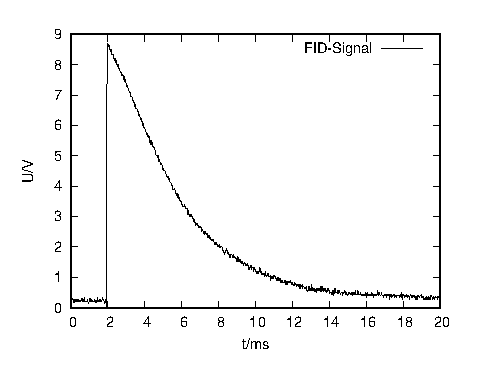
\includegraphics[width=0.75\linewidth]{data/p402_443_data/FID_1/FID_1.eps}
  \caption{FID Signal}
  \label{fig:FID}
\end{figure}


\printbibliography

\end{document}
